\documentclass[border=5mm]{standalone}
\usepackage{tikz}
\usepackage{tikz-qtree}
\usepackage{ctex}
\usetikzlibrary{calc}
\usetikzlibrary{positioning}

\tikzset{squarenode/.style={draw, rectangle, minimum size=0.7cm}}

\begin{document}
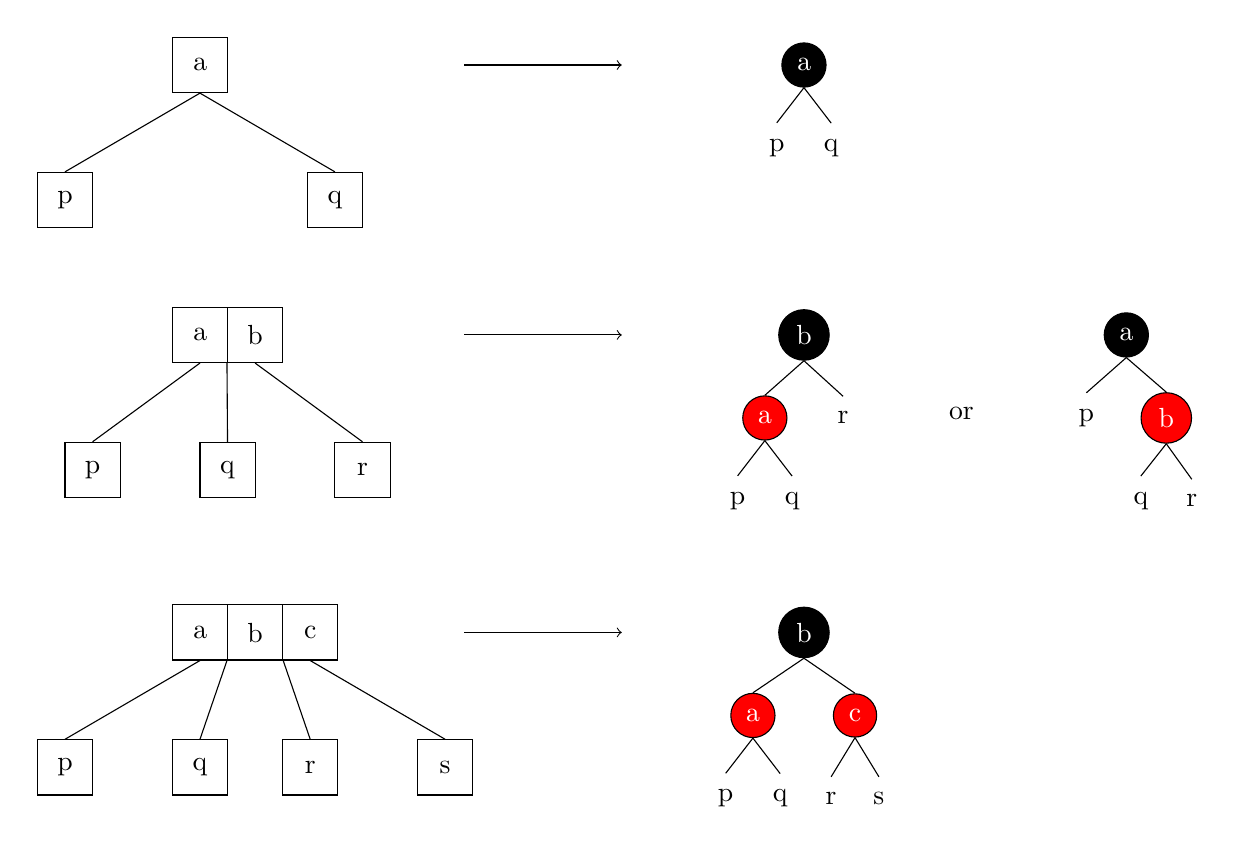
\begin{tikzpicture}[every tree node/.style={align=center}]
    \matrix[row sep=1cm, column sep=1cm] {

    \node[squarenode] (a1) {a};

    \node[squarenode, below left=of a1] (p) {p};
    \node[squarenode, below right=of a1] (q) {q};

    \draw (a1.south) -- (p.north);
    \draw (a1.south) -- (q.north);

    \draw[->] ($(a1.east) + (3, 0)$) -- +(2cm, 0);
    &
    \Tree
    [.\node[draw, fill=black, circle]{\textcolor{white}{a}};
    [.\node[draw=none, circle]{p};]
    [.\node[draw=none, circle]{q};]
    ];
    \\

    \node[squarenode] (a2) {a};
    \node[squarenode, right=-\pgflinewidth of a2] (b) {b};

    \node[squarenode, below=of $(a2.south)!0.5!(b.south)$] (q) {q};
    \node[squarenode, left=of q] (p) {p};
    \node[squarenode, right=of q] (r) {r};

    \draw (a2.south) -- (p.north);
    \draw (b.south west) -- (q.north);
    \draw (b.south) -- (r.north);

    \draw[->] ($(a2.east) + (3, 0)$) -- +(2cm, 0);
    &
    \Tree
    [.\node[draw, fill=black, circle]{\textcolor{white}{b}};
    [.\node[draw, fill=red, circle]{\textcolor{white}{a}};
    [.\node[draw=none, circle]{p};]
    [.\node[draw=none, circle]{q};]
    ]
    [.\node[draw=none, circle]{r};]
    ];
    \node at (2,-1) {or};
    &
    \Tree
    [.\node[draw, fill=black, circle]{\textcolor{white}{a}};
    [.\node[draw=none, circle]{p};]
    [.\node[draw, fill=red, circle]{\textcolor{white}{b}};
    [.\node[draw=none, circle]{q};]
    [.\node[draw=none, circle]{r};]
    ]
    ];
    \\

    \node[squarenode] (a3) {a};
    \node[squarenode, right=-\pgflinewidth of a3] (b) {b};
    \node[squarenode, right=-\pgflinewidth of b] (c) {c};

    \node[squarenode, below=of a3] (q) {q};
    \node[squarenode, left=of q] (p) {p};
    \node[squarenode, below=of c] (r) {r};
    \node[squarenode, right=of r] (s) {s};

    \draw (a3.south) -- (p.north);
    \draw (b.south west) -- (q.north);
    \draw (c.south) -- (s.north);
    \draw (b.south east) -- (r.north);

    \draw[->] ($(a3.east) + (3, 0)$) -- +(2cm, 0);
    &
    \Tree
    [.\node[draw, fill=black, circle]{\textcolor{white}{b}};
    [.\node[draw, fill=red, circle]{\textcolor{white}{a}};
    [.\node[draw=none, circle]{p};]
    [.\node[draw=none, circle]{q};]
    ]
    [.\node[draw, fill=red, circle]{\textcolor{white}{c}};
    [.\node[draw=none, circle]{r};]
    [.\node[draw=none, circle]{s};]
    ]
    ];
    \\
    };
\end{tikzpicture}
\end{document}
